\documentclass[onepage]{beamer}
\mode<presentation>{
	\setbeamercovered{transparent}
	%\beamertemplatenavigationsymbolsempty
	\setbeamertemplate{footline}[frame number]
% 	\usefonttheme{professionalfonts}
}

% https://tex.stackexchange.com/questions/34166/understanding-minipages-aligning-at-top
\usepackage{adjustbox}

% https://tex.stackexchange.com/questions/124256/how-do-i-get-numbered-entries-in-a-beamer-bibliography
\setbeamertemplate{bibliography item}{\insertbiblabel}

% https://tex.stackexchange.com/questions/49048/how-to-cite-one-bibentry-in-full-length-in-the-body-text
\usepackage{bibentry}
\bibliographystyle{plain}
\nobibliography*
%
% https://tex.stackexchange.com/questions/163827/wrong-vertical-spaces-using-bibentry-within-beamer/163842
\def\mybeamernewblock{%
  \usebeamercolor[fg]{bibliography entry author}%
  \usebeamerfont{bibliography entry author}%
  \usebeamertemplate{bibliography entry author}%
  \def\newblock{%
    \usebeamercolor[fg]{bibliography entry title}%
    \usebeamerfont{bibliography entry title}%
    \usebeamertemplate{bibliography entry title}%
    \def\newblock{%
      \usebeamercolor[fg]{bibliography entry location}%
      \usebeamerfont{bibliography entry location}%
      \usebeamertemplate{bibliography entry location}%
      \def\newblock{%
        \usebeamercolor[fg]{bibliography entry note}%
        \usebeamerfont{bibliography entry note}%
        \usebeamertemplate{bibliography entry note}}}}%
  \leavevmode
}
\newenvironment{references}{\begin{itemize}\let\newblock\mybeamernewblock}{\end{itemize}}


\setbeamersize{text margin left=10pt, text margin right=10pt}
\setbeamertemplate{itemize items}[circle]

\beamertemplatenavigationsymbolsempty

% http://tex.stackexchange.com/questions/8680/how-can-i-insert-a-newline-in-a-framebox
%\usepackage{minibox}
%\usepackage{framed}
%\usepackage[usestackEOL]{stackengine}

% % http://tex.stackexchange.com/questions/167000/annotating-tables-with-tikz-adding-arrows
% \usepackage{color, colortbl}
\usepackage{tikz}
\tikzstyle{every picture}+=[remember picture]
%\usetikzlibrary{tikzmark, positioning, fit, shapes.misc}

%% http://tex.stackexchange.com/questions/91124/itemize-removing-natural-indent
%\usepackage{enumitem}

%% http://tex.stackexchange.com/questions/41408/a-five-level-deep-list
%\usepackage{enumitem}
%\setlistdepth{9}

% https://tex.stackexchange.com/questions/20792/how-to-superimpose-latex-on-a-picture
\usepackage{overpic}

% % http://tex.stackexchange.com/questions/32661/how-to-locate-figures-with-x-y-specified-location-in-a-presentation
% \usepackage[absolute,overlay]{textpos} % absolute positioning of stuff
% \setlength{\TPHorizModule}{1mm}
% \setlength{\TPVertModule}{1mm}

\usepackage{graphicx}
\graphicspath{{../img/}}
\AtBeginDocument{\DeclareGraphicsExtensions{.eps, .png, .gif, .pdf}}

\usepackage[makeroom]{cancel}

\usepackage[english]{babel}
\usepackage[T1]{fontenc}
\usepackage{times}

% \usepackage{amssymb}
% \usepackage{nicefrac}
% \usepackage{bbm}
% \usepackage{esint}
% \usepackage{sidecap}

\usepackage{hyperref}
% \hypersetup{pdfpagemode=FullScreen}

\newcommand{\HIDE}[1]{}

\newcommand{\skipline}{{\ }\\}

\newcommand{\EMAIL}{{\color{blue}randreev{\tiny\color{white}.\hspace{-1.5pt}}@{\tiny\color{white}.\hspace{-1.5pt}}stat.sinica.edu.tw}}

\author{\small RA}
\subject{Talks}

\newcommand{\CITE}[1]{{\footnotesize[#1]}}

% \input{definitions}

\providecommand{\DIV}{\mathop{\text{div}}}
\providecommand{\GRAD}{\mathop{\text{grad}}}

\providecommand{\IE}{\mathbb{E}}
\providecommand{\IP}{\mathbb{P}}
\providecommand{\IR}{\mathbb{R}}
\providecommand{\IZ}{\mathbb{Z}}

\providecommand{\duality}[2]{\langle #1 \rangle_{#2}}
\providecommand{\norm}[2]{\| #1 \|_{#2}}
\providecommand{\seminorm}[2]{| #1 |_{#2}}
\providecommand{\VERT}{\ensuremath{| \! | \! |}}
\newcommand{\tnorm}[2]{\VERT{#1}\VERT_{{#2}}}

\newcommand{\cA}{\mathcal{A}}
\newcommand{\cB}{\mathcal{B}}
\newcommand{\cL}{\mathcal{L}}
\newcommand{\cN}{\mathcal{N}}
\newcommand{\cT}{\mathcal{T}}
\newcommand{\cX}{\mathcal{X}}
\newcommand{\cY}{\mathcal{Y}}

\providecommand{\Abf}{\mathbf{A}}
\providecommand{\Bbf}{\mathbf{B}}
\providecommand{\Dbf}{\mathbf{D}}
\providecommand{\Ibf}{\mathbf{I}}
\providecommand{\Jbf}{\mathbf{J}}
\providecommand{\Fbf}{\mathbf{F}}
\providecommand{\Hbf}{\mathbf{H}}
\providecommand{\Mbf}{\mathbf{M}}
\providecommand{\Tbf}{\mathbf{T}}
\providecommand{\Pbf}{\mathbf{P}}
\providecommand{\Vbf}{\mathbf{V}}
\providecommand{\pbf}{\mathbf{p}}
\providecommand{\ubf}{\mathbf{u}}
\providecommand{\vbf}{\mathbf{v}}
\providecommand{\wbf}{\mathbf{w}}
\providecommand{\ybf}{\mathbf{y}}
\providecommand{\zbf}{\mathbf{z}}

\renewcommand{\vec}[1]{\mathbf{#1}}

\providecommand{\T}{\mathsf{T}}

\renewcommand{\hat}[1]{\widehat{#1}}
\renewcommand{\tilde}[1]{\widetilde{#1}}

\newcommand{\rd}{\,\mathrm{d}}

\newcommand{\TEXT}[1]{\quad\text{#1}\quad}

% http://tex.stackexchange.com/questions/211518/beamer-vfill-and-itemize
\def\Bottom#1{\vskip 0pt plus 1filll #1}
\def\BottomRight#1{\Bottom{\hfill #1}}

% MATLAB CODE LISTING
\usepackage{color}
\definecolor{DarkBlue}{rgb}{0,0,0.4}
% \definecolor{DarkRed}{rgb}{0.3,0,0}
\definecolor{DarkGreen}{rgb}{0,0.3,0}
\usepackage{listings}
\lstset{%
	language=MATLAB,
	basicstyle=\bf\ttfamily\tiny,%\footnotesize,
	keywordstyle=\color{DarkBlue},
	numbers=left, numberstyle=\footnotesize, numbersep=4pt,
	commentstyle={\color{DarkGreen}},
% 	backgroundcolor=\color{white},
	showspaces=false, showstringspaces=false, showtabs=false,
	frame=none,
	tabsize=4,
	breaklines=true, breakatwhitespace=false,
	emph={[1]femT_,femT_assemE,femT_assemF,femT_assemFE,femTX_assemLoad,spacetime},
	emphstyle={[1]\color{blue}},
	emph={[2]femX_,femX_MA,femX_b,femX_init,femX_show},
	emphstyle={[2]\color{DarkGreen}},
	morekeywords={parfor,true,false},
	xleftmargin=8pt,
	numbers=none
}


%%%%%%%%%%%%%%%%%%%%%%%%%%%%%%%%%%%%%%%%%%%%%%%%%%%%%%%%%%%%%%%%%%%%%%%%%%%%%%%%
%%
%%%%%%%%%%%%%%%%%%%%%%%%%%%%%%%%%%%%%%%%%%%%%%%%%%%%%%%%%%%%%%%%%%%%%%%%%%%%%%%%

\usepackage{ifthen}

\newcommand{\REDBOX}[1]{
	\setlength{\fboxrule}{1pt}
	\fcolorbox{red}{SeeMeBarely}{$\displaystyle
		#1
	$}
}

\definecolor{SeeMeBarely}{RGB}{230,230,230}
\definecolor{Purple}{RGB}{128,0,128}
\definecolor{DeepPurple}{RGB}{32,0,96}
\newcommand{\ra}[1]{{\color{blue}{#1}}}
\newcommand{\cred}[1]{{\color{red}{#1}}}
\newcommand{\cblu}[1]{{\color{blue}{#1}}}
\newcommand{\cpur}[1]{{\color{Purple}{#1}}}

\DeclareMathOperator*{\argmin}{arg\,min}

\newcommand{\ItemComment}[1]{\hfill{\scriptsize(#1)\normalsize}}


% http://www.webnots.com/vibgyor-rainbow-color-codes/
\definecolor{a}{RGB}{148, 0, 211}
\definecolor{b}{RGB}{75, 0, 130}
\definecolor{c}{RGB}{0, 0, 255}
\definecolor{d}{RGB}{0, 160, 0}
\definecolor{e}{RGB}{200, 200, 0}
\definecolor{f}{RGB}{255, 127, 0}
\definecolor{g}{RGB}{255, 0, 0}
%
\definecolor{z}{RGB}{0, 0, 0}
\definecolor{w}{RGB}{255, 255, 255}

% http://tex.stackexchange.com/questions/17611/how-does-one-type-chinese-in-latex
\usepackage{CJKutf8}
\AtBeginDvi{\input{zhwinfonts}}
%
\newcommand{\REN}{\begin{CJK*}{UTF8}{gbsn}人\end{CJK*}}
\newcommand{\ren}[1]{{\color{#1}\REN}}



%%%%%%%%%%%%%%%%%%%%%%%%%%%%%%%%%%%%%%%%%%%%%%%%%%%%%%%%%%%%%%%%%%%%%%%%%%%%%%%%
\begin{document}
%%%%%%%%%%%%%%%%%%%%%%%%%%%%%%%%%%%%%%%%%%%%%%%%%%%%%%%%%%%%%%%%%%%%%%%%%%%%%%%%
%%%%%%%%%%%%%%%%%%%%%%%%%%%%%%%%%%%%%%%%%%%%%%%%%%%%%%%%%%%%%%%%%%%%%%%%%%%%%%%%

%%%%%%%%%%%%%%%%%%%%%%%%%%%%%%%%%%%%%%%%%%%%%%%%%%%%%%%%%%%%%%%%%%%%%%%%%%%%%%%%
\section{Intro}
%%%%%%%%%%%%%%%%%%%%%%%%%%%%%%%%%%%%%%%%%%%%%%%%%%%%%%%%%%%%%%%%%%%%%%%%%%%%%%%%



\begin{frame}[plain,t]
	\begin{center}
		%\small
		%
		Some stats on the GSE75688 BC dataset
		%
		\\[1\baselineskip]
		\small
		RA
% 		\\[1\baselineskip]
% 		\footnotesize
% 		ISS, AS \\ \EMAIL

		\vspace{1cm}

		%

	\end{center}

	\Bottom{
		\scriptsize
		%Support: 
		\hfill
		Dec, 2017
		\\ {\ }
	}
\end{frame}


%%%

\begin{frame}[t]{Differential expression (KS distance max/tumors)}{Hand-picked GO terms}
	\begin{center}
		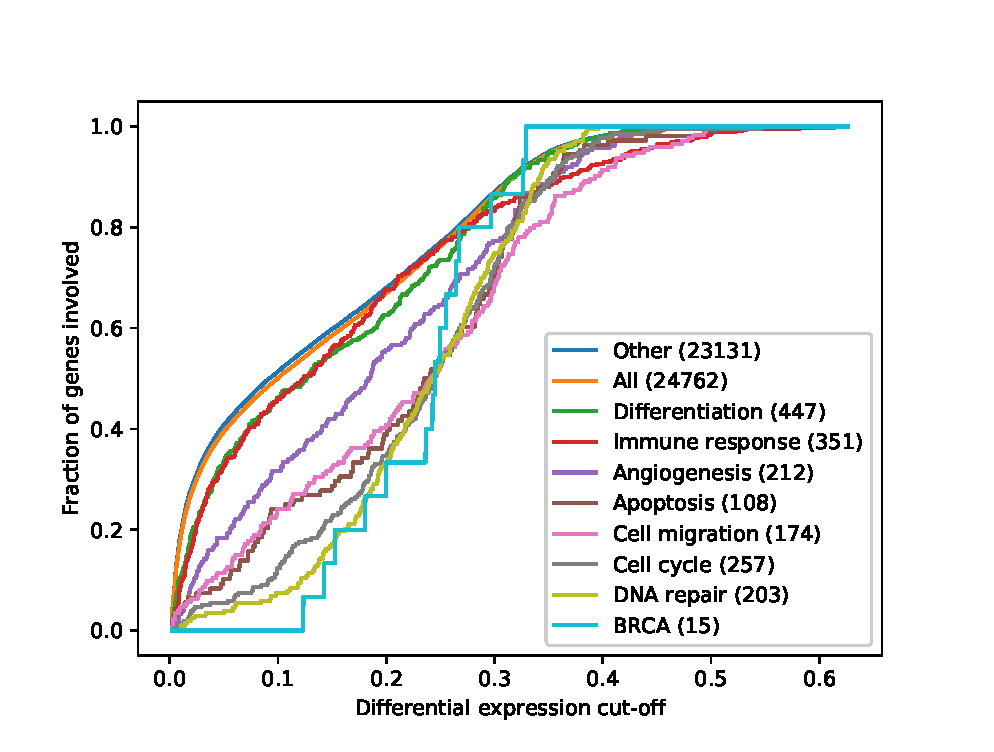
\includegraphics[width=0.9\textwidth]{3_proba_a/de2m_full}
	\end{center}
\end{frame}

%%%

\begin{frame}[t]{Differential expression (KS distance max/tumors)}{Most uniformly expressed among 400 most frequent GO terms}
	\begin{center}
		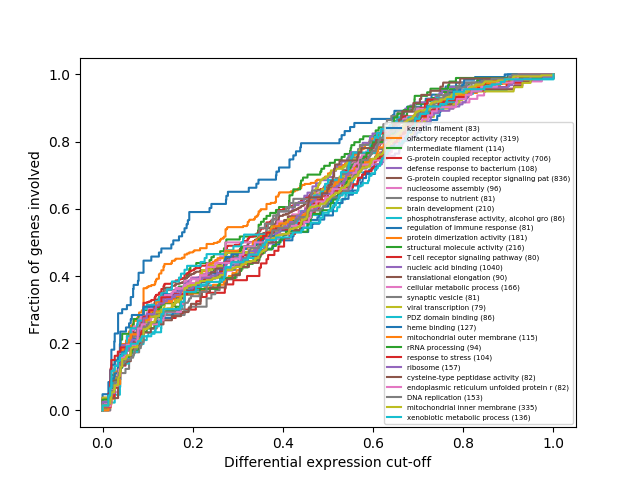
\includegraphics[width=0.9\textwidth]{3_proba_a/de2go_full}
	\end{center}
\end{frame}

%%%

\begin{frame}[t]{Sample-wise expression}{Overview}
	\begin{center}
		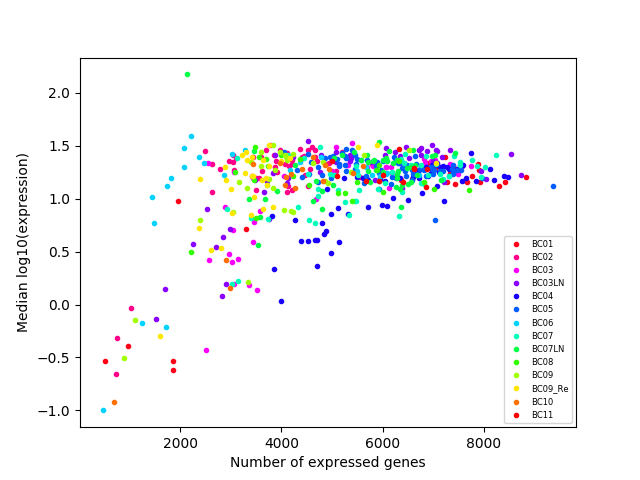
\includegraphics[width=0.9\textwidth]{2_stats_b/nnz-median}
	\end{center}
\end{frame}

%%%

\begin{frame}[t]{Expression heatmap}{}
	\begin{center}
		\includegraphics<1>[width=0.9\textwidth]{7_heatmaps/heatmap_None}
		\includegraphics<2>[width=0.9\textwidth]{7_heatmaps/heatmap_GO-0001525}
		\includegraphics<3>[width=0.9\textwidth]{7_heatmaps/heatmap_GO-0002039}
		\includegraphics<4>[width=0.9\textwidth]{7_heatmaps/heatmap_GO-0006281}
		\includegraphics<5>[width=0.9\textwidth]{7_heatmaps/heatmap_GO-0006955}
		\includegraphics<6>[width=0.9\textwidth]{7_heatmaps/heatmap_GO-0016477}
		\includegraphics<7>[width=0.9\textwidth]{7_heatmaps/heatmap_GO-0006915}
		\includegraphics<8>[width=0.9\textwidth]{7_heatmaps/heatmap_GO-0043065}
		\includegraphics<9>[width=0.9\textwidth]{7_heatmaps/heatmap_GO-0043066}
	\end{center}
	{\only<1>{All genes (24762), sorted by KS differential expression}}
	{\only<2>{GO:0001525 -- angiogenesis (234)}}
	{\only<3>{GO:0002039 -- p53 binding (68)}}
	{\only<4>{GO:0006281 -- DNA repair (363)}}
	{\only<5>{GO:0006955 -- immune response (410)}}
	{\only<6>{GO:0016477 -- cell migration (194)}}
	{\only<7>{GO:0006915 -- apoptotic process (658)}}
	{\only<8>{GO:0043065 -- positive regulation of apoptotic process (330)}}
	{\only<9>{GO:0043066 -- negative regulation of apoptotic process (486)}}
\end{frame}

%%%

\begin{frame}[t]{DE vs Signal map}{}
	\begin{center}
		\includegraphics<1>[width=0.99\textwidth]{7_heatmaps/de-vs-ex_GO-0004984}
		\includegraphics<2>[width=0.99\textwidth]{7_heatmaps/de-vs-ex_GO-0001525}
		\includegraphics<3>[width=0.99\textwidth]{7_heatmaps/de-vs-ex_GO-0002039}
		\includegraphics<4>[width=0.99\textwidth]{7_heatmaps/de-vs-ex_GO-0006281}
		\includegraphics<5>[width=0.99\textwidth]{7_heatmaps/de-vs-ex_GO-0006955}
		\includegraphics<6>[width=0.99\textwidth]{7_heatmaps/de-vs-ex_GO-0016477}
		\includegraphics<7>[width=0.99\textwidth]{7_heatmaps/de-vs-ex_GO-0006915}
		\includegraphics<8>[width=0.99\textwidth]{7_heatmaps/de-vs-ex_GO-0043065}
		\includegraphics<9>[width=0.99\textwidth]{7_heatmaps/de-vs-ex_GO-0043066}
	\end{center}
	%{\only< 1>{All genes (24762)}}
	{\only<1>{GO:0004984 -- olfactory receptor activity (150)}}
	{\only<2>{GO:0001525 -- angiogenesis (234)}}
	{\only<3>{GO:0002039 -- p53 binding (68)}}
	{\only<4>{GO:0006281 -- DNA repair (363)}}
	{\only<5>{GO:0006955 -- immune response (410)}}
	{\only<6>{GO:0016477 -- cell migration (194)}}
	{\only<7>{GO:0006915 -- apoptotic process (658)}}
	{\only<8>{GO:0043065 -- positive regulation of apoptotic process (330)}}
	{\only<9>{GO:0043066 -- negative regulation of apoptotic process (486)}}
\end{frame}

%%%

\begin{frame}[t]{Genes with low DE by signal strength}{}
	\begin{center}
		\includegraphics<1>[width=0.99\textwidth]{7_heatmaps/ex-sect_8-}
		\includegraphics<2>[width=0.99\textwidth]{7_heatmaps/ex-sect_9-}
		\includegraphics<3>[width=0.99\textwidth]{7_heatmaps/ex-sect_10-}
		\includegraphics<4>[width=0.99\textwidth]{7_heatmaps/ex-sect_11-}
		\includegraphics<5>[width=0.99\textwidth]{7_heatmaps/ex-sect_12-}
		\includegraphics<6>[width=0.99\textwidth]{7_heatmaps/ex-sect_13-}
% 		\includegraphics<7>[width=0.99\textwidth]{7_heatmaps/ex-sect_14-}
% 		\includegraphics<8>[width=0.99\textwidth]{7_heatmaps/ex-sect_15-}
% 		\includegraphics<9>[width=0.99\textwidth]{7_heatmaps/ex-sect_16-}
	\end{center}
\end{frame}

%

\begin{frame}[t]{}{}
	\scriptsize
	{\only<1>{%
		``lytic vacuole'' (GO:0000323)
		\begin{itemize}
		\item
			The lytic vacuole is a plant specialized vacuole equivalent to animal lysosomes or yeast vacuoles, functioning as compartments for degradation and waste storage. 
			\\
			{\tiny \url{http://www.uniprot.org/locations/SL-0159}}
		\item
			``We focus on targeting the lysosome in cancer by exploring lysosomal biogenesis and its role in the crosstalk between apoptosis and autophagy. We also discuss how lysosomal inhibition could emerge as a new therapeutic strategy to overcome drug resistance in cancer.''
			\\
			{\tiny \url{https://www.ncbi.nlm.nih.gov/pmc/articles/PMC4879098/} }
		\item
			``Lysosomes, with their arsenal of degradative enzymes are increasingly becoming an area of interest in the field of oncology. The changes induced in this compartment upon transformation are numerous and whereas most are viewed as pro-oncogenic the same processes also render cancer cells susceptible to lysosomal death pathways.''
			\\
			{\tiny \url{https://www.sciencedirect.com/science/article/pii/S0167488908003170}}
		\end{itemize}
	}}%
	{\only<2>{%
		``Ser-tRNA(Ala) hydrolase activity'' (GO:0002196)
		\begin{itemize}
		\item
			``We compare genome-wide tRNA expression in cancer-derived versus non-cancer-derived breast cell lines, as well as tRNA expression in breast tumors versus normal breast tissues. In cancer-derived versus non-cancer-derived cell lines, nuclear-encoded tRNAs increase by up to 3-fold and mitochondrial-encoded tRNAs increase by up to 5-fold. In tumors versus normal breast tissues, both nuclear- and mitochondrial-encoded tRNAs increase up to 10-fold.''
			\\
			{\tiny \url{https://www.ncbi.nlm.nih.gov/pmc/articles/PMC2790902/}}
		\end{itemize}
	}}%
	{\only<3>{%
		``lymphocyte chemotaxis across high endothelial venule'' (GO:0002518)
		\begin{itemize}
		\item
			``High endothelial venules (HEV) are specialized post-capillary venous swellings characterized by plump endothelial cells as opposed to the usual thinner endothelial cells found in regular venules. HEVs enable lymphocytes circulating in the blood to directly enter a lymph node (by crossing through the HEV).''
			\\
			{\tiny \url{https://en.wikipedia.org/wiki/High_endothelial_venules}}
		\item
			``Chemotaxis not only affects tumour cells but also helps to shape the tumour microenvironment. Directional migration to a chemokine source is evident both in vitro and in vivo for most of the cells of the tumour microenvironment. Epithelial cells produce multiple factors that recruit various tumour-infiltrating cells, including tumour-associated macrophages (TAMs), tumour-associated neutrophils (TANs), lymphocytes, cancer-associated fibroblasts (CAFs), mesenchymal stem cells (MSCs) and endothelial cells.''
			\\
			{\tiny \url{https://www.ncbi.nlm.nih.gov/pmc/articles/PMC4030706/}}
		\end{itemize}
	}}%
	{\only<4>{%
		``intracellular defense response'' (GO:0002818)
		\begin{itemize}
		\item --
		\end{itemize}
	}}%
	{\only<5>{%
		``estrone sulfotransferase activity'' (GO:0004304)
		\begin{itemize}
		\item
			``This enzyme participates in androgen and estrogen metabolism and sulfur metabolism.''
			\\
			{\tiny \url{https://en.wikipedia.org/wiki/Estrone_sulfotransferase}}
		\item
			``Estrone sulfate (E1S) is concentrated in high levels in human breast cancer tissue. The values are particularly high in postmenopausal women and many times those circulating in the plasma. Also, the tissular concentration of this conjugate are significantly higher in tumoural tissue than in the area of the breast considered as normal. The enzyme which hydrolyzes E1S: sulfatase, as well as the enzyme which biosynthesises this conjugate: sulfotransferase, are present in significant concentrations in breast cancer tissue.''
			\\
			{\tiny \url{https://www.ncbi.nlm.nih.gov/pubmed/10419004}}
		\end{itemize}
	}}%
	{\only<6>{%
		``hypoxanthine phosphoribosyltransferase activity'' (GO:0004422)
		\begin{itemize}
		\item
			``Hypoxanthine-guanine phosphoribosyltransferase (HGPRT) is an enzyme encoded in humans by the HPRT1 gene. [..] HGPRTase functions primarily to salvage purines from degraded DNA to reintroduce into purine synthetic pathways.''
			\\
			{\tiny \url{https://en.wikipedia.org/wiki/Hypoxanthine-guanine_phosphoribosyltransferase}}
		\item
			``This enzyme plays a central role in the generation of purine nucleotides through the purine salvage pathway. Mutations in this gene result in Lesch-Nyhan syndrome or gout.''
			\\
			{\tiny \url{https://www.proteinatlas.org/ENSG00000165704-HPRT1/pathology}}
		\end{itemize}
	}}%
	{\only<7>{%
		``collagen type III trimer'' (GO:0005586)
		\begin{itemize}
		\item
			``Type III collagen, which adds structure and strength to connective tissues, is found in many places in the body, especially skin, lung, intestinal walls, and the walls of blood vessels. Collagen III is initially produced as procollagen, a protein consisting of three pro-alpha1(III) chains that form the triple-stranded, rope-like molecule. After being synthesized, the procollagen molecule is modified by the cell.''
			\\
			{\tiny \url{http://www.merckmillipore.com/product/Human-Collagen-Type-III,MM_NF-CC054}}
		\item
			``Increased synthesis and degradation of extracellular matrix components are associated with breast cancer development. This study evaluated type I and type III procollagen mRNA expression and the corresponding protein synthesis and maturation, as well as the tissue distribution of these collagens, [..]. In the benign lesions, the type I and type III collagen bundles were regularly organized and the expression of the corresponding mRNA was weak, indicating a relatively slow collagen turnover. In the malignant tumours, increased expression of type I and type III procollagen mRNAs was observed in the fibroblastic cells of the stroma; the malignant epithelial cells did not participate. [..] Metastases of breast carcinoma resembled poorly differentiated primary tumours with respect to their collagen synthesis and deposition. The increased synthesis of fibrillar type I and type III procollagens may serve as a pathway for tumour invasion. The enhanced synthesis is associated with the formation of aberrant collagen bundles, which may be more readily degradable and may thus facilitate breast tumour invasion.''
			\\
			{\tiny \url{https://www.ncbi.nlm.nih.gov/pubmed/10211114}}
		\end{itemize}
	}}%
\end{frame}


%%%%%%%%%%%%%%%%%%%%%%%%%%%%%%%%%%%%%%%%%%%%%%%%%%%%%%%%%%%%%%%%%%%%%%%%%%%%%%%%%
%\section{Extra}
%%%%%%%%%%%%%%%%%%%%%%%%%%%%%%%%%%%%%%%%%%%%%%%%%%%%%%%%%%%%%%%%%%%%%%%%%%%%%%%%%
%
%
\newcounter{finalframe}
\setcounter{finalframe}{\value{framenumber}}
% Backup frames follow
%
%
%\begin{frame}
%	Appendix
%\end{frame}
%
%%
%
%\begin{frame}
%	%
%\end{frame}
%
%
% FINAL SLIDE
\setbeamercolor{background canvas}{bg=black}
\begin{frame}[plain,b]
	\hfill
	\tiny
	\color{gray}
	this slide is intentionally left blank
\end{frame}
\setbeamercolor{background canvas}{bg=white}


%%%%%%%%%%%%%%%%%%%%%%%%%%%%%%%%%%%%%%%%%%%%%%%%%%%%%%%%%%%%%%%%%%%%%%%%%%%%%%%%%
%\section{Bibliography}
%%%%%%%%%%%%%%%%%%%%%%%%%%%%%%%%%%%%%%%%%%%%%%%%%%%%%%%%%%%%%%%%%%%%%%%%%%%%%%%%%

% {
% \tiny
% \bibliography{../../../r/refs}
% }


%%%%%%%%%%%%%%%%%%%%%%%%%%%%%%%%%%%%%%%%%%%%%%%%%%%%%%%%%%%%%%%%%%%%%%%%%%%%%%%%
\setcounter{framenumber}{\value{finalframe}}
\end{document}
%%%%%%%%%%%%%%%%%%%%%%%%%%%%%%%%%%%%%%%%%%%%%%%%%%%%%%%%%%%%%%%%%%%%%%%%%%%%%%%%
%%%%%%%%%%%%%%%%%%%%%%%%%%%%%%%%%%%%%%%%%%%%%%%%%%%%%%%%%%%%%%%%%%%%%%%%%%%%%%%%

